\documentclass[../entwurf.tex]{subfiles}

\begin{document}
\section{Sequenzdiagramme}
\subsection{Starten eines Songs aus der Audiobibliothek}
\begin{center}
	\includegraphics[page=1,width=350pt,keepaspectratio]{../graphics/sequenz_diagramme/PlaySongSequenzDia.png}
\end{center}
Das Sequenz-Diagramm stellt dar was passiert nachdem der User auf einen Song in der AudioLibrary gedrückt hat.

\subsection{Suchen neuer ESense Earables}
Das folgende Sequenz-Diagramm stellt dar was passiert, wenn der User auf der ConnectionPage auf den Refresh-Button drückt.
\begin{center}
	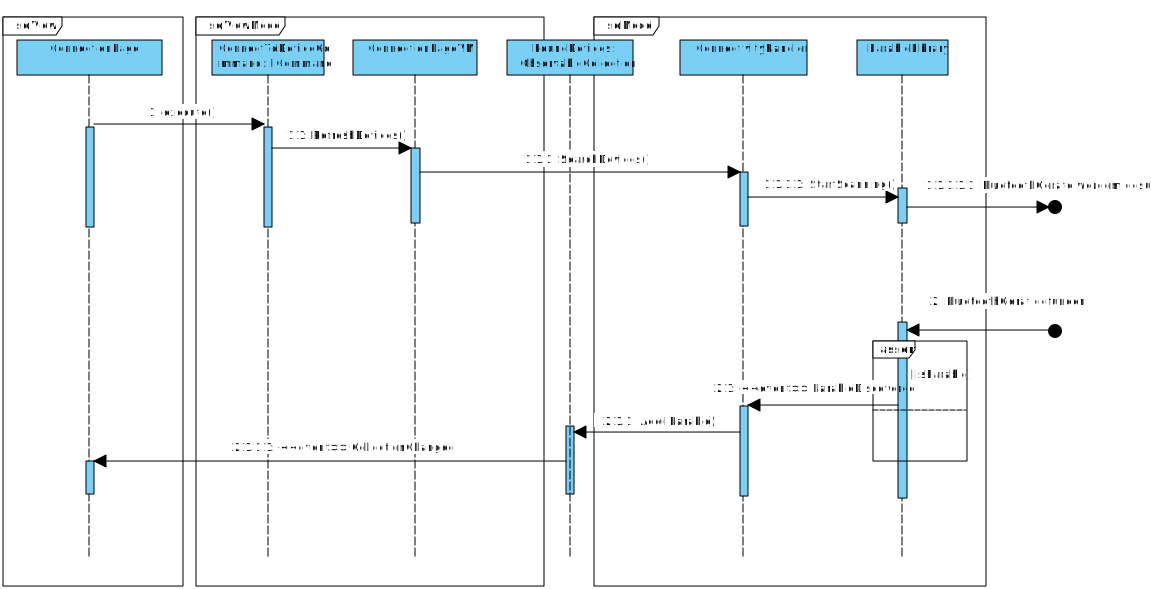
\includegraphics[page=1,width=350pt,keepaspectratio]{../graphics/sequenz_diagramme/RefreshFoundDevices.png}
\end{center}
\paragraph{Beschreibung}
Die View-Klasse \code{ConnectionPage} führt (unter Anwendung von \Gls{databinding}) einen dafür vorgesehenen \code{ICommand} aus dem ViewModel aus (\code{execute()}).
Dies führt zu einem Ausführen von \code{RefreshDevices()} in der \code{ConnectionsPageVM},
was wiederum einen Aufruf von \code{SearchDevices()} in der Model-Klasse \code{ConnectivityHandler} induziert.
Dies wiederum startet den Suchvorgang in der \code{EarableLibrary} (\code{StartScanning()}).
Im weiteren führt das Betriebssystem eine Suche nach Bluetooth-Geräten aus.
Für jedes derart gefundenes Gerät überprüft die \code{EarableLibrary} zunächst, ob es sich dabei um ein Earable-Gerät handelt.
Ist dem so, wird mittels \Gls{event} (\code{EarableDiscovered}) der \code{ConnectvitiyHandler} aufgerufen.
Dieser verwaltet eine interne Liste (\code{FoundDevices}), welche alle aktuell in der Nähe befindlichen Earables auflistet.
Da es sich hierbei um eine \code{ObservableCollection} handelt - welche durch eine weitergeleitete \Gls{property} im ViewModel auch der View zur Verfügung steht -
kann diese durch ein weiteres \Gls{event} (\code{CollectionChanged}) über die Änderung informiert werden und das neue Gerät anzeigen.

\subsection{Aktivieren eines Modus}
\begin{center}
	\includegraphics[page=1,width=350pt,keepaspectratio]{../graphics/sequenz_diagramme/ActivateModeDia.png}
\end{center}
Das Diagramm stellt dar was passiert wenn der User auf die ModePage wechselt und einen beliebigen Modus der App aktiviert.

\subsection{Verwendung des AutoStop Modus}
\begin{center}
	\includegraphics[page=1,width=350pt,keepaspectratio]{../graphics/sequenz_diagramme/AutoStopDia.png}
\end{center}
Das Sequenz-Diagramm stellt dar was passiert wenn der User bei gestartetem AutoStop-Modus das Laufen unterbricht und stehen bleibt.

\end{document}
